\section{Optimization}
\label{sec:concept_optimization}
Our compiler does not only translate the source language Luie to the target language OpenQASM but can also apply optimizations to the program. Since quantum programs must be deterministic and, therefore, most language constructs are translated at compile time, many classical optimizations are inherently applied. The following, inherent optimizations are discussed generally in Sec.~\ref{sec:background_codeOptimization}.

The first kind of inherent optimizations are constant propagation and constant folding. 
While the target language does allow for expressions, they need to be constant. Furthermore, some language features that depend on expressions have no equivalent in the target language. In turn, they, and their corresponding expressions, need to be evaluated at compile time. This is the case for, \eg, the control flow statements. Therefore, any variable is always constant and its value is propagated to be used in the evaluation of expressions. Further, each expression is evaluated at compile time such that constant propagation and constant folding are inherently applied.

Secondly, loop unrolling is always applied to all loop statements. OpenQASM does not allow for loop statements or any other method for the iteration of statements, besides the restrictive implicit iteration. Furthermore, quantum computers in general cannot provide the ability to iterate over gates since they operate on static circuits. Therefore, to allow for loop statements in our language, the loop is unrolled entirely at compile time. Additionally, for each iteration the current value of the loop iterator is propagated as a constant through the loop body.   

The last inherent optimization is function inlining. Our language provides the ability to define custom gates that consist of an arbitrary combination of gate applications and, possibly, control flow statements. While OpenQASM has a similar functionality, the composite gates OpenQASM provides are more restrictive; for example, they do not allow for registers as arguments to the gate. Furthermore, in contrast to classical computers, quantum computers do not natively support function calls or related concepts. Therefore, each time a composite gate is used, the compiler inlines the gate body at the location where the gate is applied.   

\subsection{Optimization Rules}
\label{sec:concept_optimizationRules}
After the code is translated, the compiler can perform additional peephole optimizations; these are not inherent to the translation of the program and, therefore, are optional. 
The peephole optimizations can be applied to the internal representation of the source language and most hardware-independent optimizations are usually applied to the intermediate representation instead of the target language. However, the peephole optimization rules only operate on sequences of gate applications such that control flow statements or composite gates may only hinder, not aid, the effectiveness of the optimization. The overall performance of the optimization may be increased by optimizing composite gates before inlining their code so that a gate that is called ten times only needs to be optimized once; nevertheless, inlining the gates before applying the rules may enable more optimizations and, thereby, increase the effectiveness at the cost of performance. Therefore, we apply the optimization rules after the code is translated.
% \todo{Why do we need to apply to translated code and not intermediate? most optimizations typically on intermediate} 
Additionally, the user can not only specify whether optimizations are applied but also which to apply when using the compiler. In the following section, we discuss the different peephole optimization rules. 
Additionally, while some optimizations are referred to by the terms commonly used in literature, as described in Sec.~\ref{sec:background_circuitOptimization}, the others without any naming conventions are given descriptive names.
% Additionally, the theoretical background for the rules is discuss in Sec.~\ref{sec:background_circuitOptimization}.

The first kind of optimization rules are the \emph{null gate} optimizations; they describe sequences of gate applications such that the resulting behavior is equivalent to applying the identity gate. In the case of classical computers, an example is the sequential execution of two negation operations. In contrast, a quantum example is the application of two successive Hadamard gates. While these optimizations can easily be performed by the programmer themselves for a simple list of instructions, the manual optimizations increase in complexity when using composite gates and control flow statements. Moreover, the programmer cannot remove two null gates by hand that are contained in two different successive composite gates. Therefore, the optimization rules can not only help to reduce the workload of the programmer but apply optimization rules that cannot be implemented without major changes to the program.

Next, the \emph{peeping control} optimization rule also belongs to the null gate rules. However, its implementation requires some additional evaluations and, therefore, we separate it from the other null gate rules. The peeping control rule can remove a controlled gate from the circuit if the value of the control wire is $\ket{0}$ at the position of the gate. To estimate the value of the control wire, the implementation needs to iterate over all previous gates on the wire. Therefore, while it is still a null gate, its implementation differs greatly from the other null gates. Furthermore, we implement an additional optimization that removes the control from the gate if the value of the control wire is known to be $\ket{1}$. While the rule does not reduce the gate count of the circuit, it may enable further optimizations on the control wire. For example, two $X$ gates on the control wire can be separated by a controlled-not gate. If the value of the control is $\ket{1}$ when the controlled-not gate is applied, the control can be removed and the now successive $X$ gates can be removed with a null gate optimization. Since this optimization does not remove the gate from the circuit, it is not a null gate optimization.

Another optimization rule that the compiler implements is the \emph{Hadamard reduction} rule. It implements the matrix equivalences for both the $X$ and $Z$ gates being surrounded by Hadamard gates, $HXH = Z$ and $HZH = X$. Thereby, the rule reduces the gate count of the circuit if the optimization rule is applied. However, the optimization rule does not remove the gate combination but replaces it with another; therefore, the rule is not a null gate optimization. 
%\change{Dont like the description, cannot come up with better right now}
Similar to the null gate optimizations, the rules themselves are not hard to apply by hand. However, in combination with the more complex statements available in the language, the application of the rule is not trivial and the compiler can optimize parts of the circuit that would have required major changes to optimize them manually.

Lastly, the \emph{control reversal} optimization rule optimizes a controlled-not gate that is surrounded by Hadamard gates on both the control and target wires. When applied, the four Hadamard gates are removed and the control and target qubits of the gate are switched. Therefore, the gate count is reduced by four gates. As described in Sec.~\ref{sec:background_circuitOptimization}, the optimization is based on two Hadamard reductions and the control reversal of the controlled-$Z$ gate. However, the reversal of the controlled-$Z$ gate does not have any direct gain when applied; it can only enable other optimizations. Furthermore, the application of the controlled-$Z$ reversal may also disabled other optimizations. Therefore, an optimization algorithm using the rule would need to either test both possibilities or estimate the value of the application and, in turn, increase the complexity of the optimization algorithm significantly. Because of this, our optimizations do not include the controlled-$Z$ reversal but implement only the special use case of the rule, the control reversal optimization rule.

\subsection{Circuit Graph}
\label{sec:concept_circuitGraph}
While it is possible to directly apply optimizations to the program code or internal representation of the code, this approach can be tedious and error prone. For example, the easiest approach would be to iterate over the code and search for code sequences with more efficient but equivalent alternatives, similar to the peephole optimization patterns on classical computers presented in Sec.~\ref{sec:background_codeOptimization}. However, two consecutive gates operating on a single wire may be separated by multiple gate applications on different wires in the programmatic description. 
Therefore, many simple optimization rules may not be applied when using a simplistic algorithm. A more complex approach would be to subdivide the program into lists of gate applications where the wires, being operated on by each list, are disjunct. While this approach can result in the application of more optimization rules, it will also miss possible applications and already requires a complex implementation. Furthermore, improving on this method only increases its complexity and, in turn, makes it more prone to errors and generally tedious to work with and debug. Therefore, the language does not directly apply the optimizations to the program but uses a circuit graph description, based on the graph described by Kreppel et al.~\cite{KMO*23}, to apply the optimizations.

The circuit graph $C$ is a graphical description of a quantum circuit; it is an acyclic and directed graph. Furthermore, it is an extension of the classical graph definition. Therefore, besides the set of nodes $V$ and edges $E$, it includes a set of qubits $Q$ associated with the graph, and relations between input, output nodes and qubit $Q_V$ as well as the edges and qubits $Q_E$. The set of nodes $V$ consists of the set of input nodes $I$, output nodes $O$, and gate nodes $G$.
\begin{align*}
    C &= (V, E, Q, Q_E, Q_V)\\
    V &= \underbrace{I}_{\text{Input Nodes}} \cup \underbrace{O}_{\text{Output Nodes}} \cup \underbrace{G}_{\text{Gate Nodes}}\\
    E &\subseteq \{ (x, y) \mid x,y \in V \land x \neq y \}\\
    Q_E &\subseteq \{ (e, q) \mid e \in E \land q \in Q \}\\
    Q_V &\subseteq \{ (v, q) \mid v \in I \cup O \land q \in Q \}
\end{align*}
For each qubit in the circuit, there exists both an input node and an output node and each input-output node pair is assigned exactly one qubit.
Furthermore, input nodes do not have an incoming edge while output nodes do not have an outgoing edge. 
Moreover, each input node has exactly one outgoing edge while each output node has exactly one incoming edge; the qubits assigned to the outgoing or incoming edges are the same as the qubits assigned to the corresponding input or output nodes.  
\begin{align*}
    \forall q \in Q :\ & (\exists_{=1} i \in I \text{ such that } (i, q) \in Q_V) \land\\
                       & (\exists_{=1} o \in O \text{ such that } (o, q) \in Q_V) \\
    \forall i \in I :\ & \nexists v \in V \text{ such that } (v, i) \in E\\
                       & (\exists_{=1} v \in (O \cup G) \text{ such that } (i, v) \in E  \ \land\\
                       & (\exists_{=1} q \in Q \text{ such that } (i, q) \in Q_V \ \land \\
                       &  ((i, v), q) \in Q_E))\\
    \forall o \in O :\ & \nexists v \in V \text{ such that } (o, v) \in E\\
                       & (\exists_{=1} v \in (I \cup G) \text{ such that } (v, o) \in E \ \land\\
                       & (\exists_{=1} q \in Q \text{ such that } (o, q) \in Q_V \ \land \\
                       &  ((v, o), q) \in Q_E))
\end{align*}

Besides the input and output nodes, all other nodes represent gates in the circuit. For all gate nodes, the number of incoming edges is equivalent to the number of outgoing edges. Additionally, the number of incoming, or outgoing, edges is the same as the number of arguments for the gate. 
Importantly, in this case, any qubits controlling the application of the gate, \eg the first qubit in a controlled-not gate, also count to the number of arguments. 
\begin{align*}
    \forall g \in G :\ & |g| = 2n \quad \text{where } n \text{ Number of arguments for gate of } g
\end{align*}
Each edge is assigned exactly one qubit. Furthermore, for all gate nodes, each incoming edge has a corresponding outgoing edge with the same assigned qubit.
\begin{align*}
    \forall e \in E :\ & (\exists_{=1} q \in Q \text{ such that } (e, q) \in Q_E)\\
    \forall v \in G :\ & (\exists v': (v', v) \in E) \implies\\
    & (\exists q, v'' : ((v', v), q) \in Q_E \land (v, v'') \in E \land ((v, v''), q) \in Q_E)
\end{align*}
Therefore, for each qubit, there exists one path from its input node to its output node such that all gates that are applied to it are visited in order of application.

\subsubsection{Graph Construction}
When using the circuit graph to optimize a quantum program, the first step is to systematically construct the graph from the program. The creation of the graph starts with the input and output nodes for each qubit in the circuit. For each declaration of a qubit, an input and output node pair is created. If a register is declared, a pair is created separately for each qubit in the register, \ie for a register with size $n$, $n$ pairs are created in total. Next, the gate applications in the program can be iterated. For each gate application, a corresponding gate node is created. To insert this node into the graph, each qubit argument requires an incoming edge to this node and a corresponding outgoing edge from the node. Additionally, the incoming node must come from the gate that was previously applied to the qubit or, if no gate was applied beforehand, the input node. Similarly, the outgoing edge must lead to either the next applied gate or the corresponding output. Therefore, for each qubit, the edge coming into the output node can be diverted to the gate node and an outgoing edge, from the gate to the output node, can be created. Repeating this step for all gate applications in the program results in the corresponding circuit graph.

An example of a simple, unoptimized circuit graph is depicted in Fig.~\ref{fig:circuit_graph_unoptimized}. For simplicity, all applied gates are depicted inside of the corresponding node in the circuit graph. The circuit consists of three qubits, $q_0$, $q_1$, and $q_2$. Their input and output nodes are depicted on the left and right of the graph, respectively and are labeled with the corresponding qubit. Firstly, an $X$ gate is applied to the first qubit $q_0$. Then, a controlled-not gate is applied to the first two qubits $q_0$ and $q_1$, where $q_0$ is the control qubit. Simultaneously, two Hadamard gates $H$ are applied to the third qubit $q_2$. Lastly, another $X$ gate is applied to the first qubit $q_0$ while another controlled-not gate is applied to the second and third qubits $q_1$ and $q_2$. In this case, the second qubit $q_1$ is the control qubit.

\begin{figure}[htp]
    \centering     
    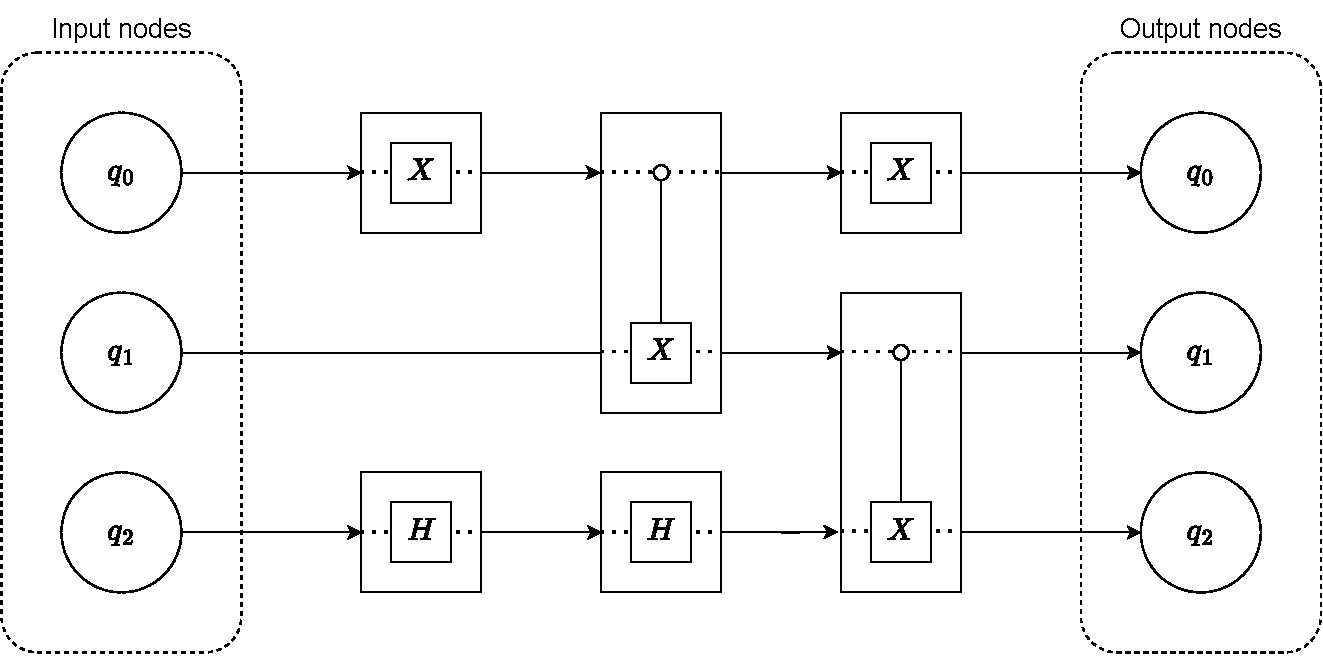
\includegraphics[width=.9\textwidth]{../figures/drawio/circuit_graph_unoptimized.pdf}
    \caption{An example of a simple, unoptimized circuit graph.}
    \label{fig:circuit_graph_unoptimized}
\end{figure}

\subsubsection{Graph Optimization}
The next step in the optimization process is the application of optimization rules. In this case, these are peephole optimizations. To optimize the graph, subgraphs are systematically iterated for each qubit $q \in Q$ by walking along the wire path of $q$. 
A wire path is a path that starts at the input node of a qubit $q$, ends in the corresponding output node, and follows the edges corresponding to the qubit $q$. 
For each node $start$ in the wire path, subpath $p$ starting at $start$ and following the wire path up to a maximum length $max$ are iterated.
This $max$ length depends on the maximum number of nodes that are affected by an optimization rule.
Each subgraph $p$ is checked for an optimized alternative based on a list of optimization rules $R$. If one is found, the subgraph is replaced with it. 
However, a single iteration over the entire graph may not find all optimizations as the application of optimizations may enable further optimizations. 
For example, after removing a gate combination, two previously separated Hadamard gates may now represent a null gate combination which can, in turn, also be removed. 
Therefore, the process needs to be repeated until no more optimizations can be applied. This is the case, if the process is repeated without applying any optimizations.
The optimization algorithm, depicted in Alg.~\ref{alg:concept_optimizationAlgorithm}, shows how the subpaths are iterated.

% Pseudo code for algorithm
\SetKwComment{Comment}{\# }{}
\begin{algorithm}
    \caption{The algorithm used to optimize a circuit graph.}
    \label{alg:concept_optimizationAlgorithm}
    \KwData{Circuit Graph $C = (V, E, Q, Q_E, Q_V)$, List of optimization rules $R$, Maximal rule length $max$}
    $repeat \gets true$\;
    \While{$repeat = true$}{
        $repeat \gets false$\;
        \ForEach(\Comment*[f]{Iterate through all qubits}){$q \in Q$}
        {
            $start \gets i \quad \text{where } (i, q) \in Q_V \land i \in I$\Comment*[r]{$I$ input nodes}
            $start \gets v \quad \text{where } ((start, v), q) \in Q_E$\Comment*[r]{Next node on wire path}
            \While(\Comment*[f]{$O$ output nodes}){$start \not\in O$}{
                $last \gets start$\;
                $p \gets [start]$ \Comment*[r]{Create path that starts with $start$}
                \For(\Comment*[f]{Iterate paths up to $max$ length}){$i \gets 0$ \KwTo $max$}{
                    \ForEach(\Comment*[f]{Check all rules for applicability}){$r \in R$}{ 
                        \If{$r$ can be applied to $p$}{
                            apply $r$ to $p$\;
                            $repeat \gets true$\;
                            $break$\;
                        }
                    }
                    \If(\Comment*[f]{Existence of next node}){$\nexists \ v : ((last, v), q) \in Q_E$}{
                        break\;
                    }
                    $last \gets v \quad \text{where } ((last, v), q) \in Q_E$\; 
                    append $last$ to $p$\;
                }
                
                $start \gets v \quad \text{where } ((start, v), q) \in Q_E$\Comment*[r]{Next node on wire path}
            }
        }
    }
\end{algorithm}

An example optimization process of a circuit graph depicted in Fig.~\ref{fig:circuit_graph_unoptimized}. Firstly, subpaths for the wire path of the first qubit $q_0$ are iterated. Here, the subpath of note is the path with the first two gate nodes $X$ and $CX$. Since the $X$ node is the child of the input node, we know that the value of the qubit will be $\ket{1}$ after the application. Therefore, we know that the controlled-not gate will always apply the $X$ gate to the second qubit $q_1$ and we can replace the $CX$ gate node with a simple $X$ node that is only visited by the second wire path. For simplicity, we assume that the optimizations are only applied after all subpaths are iterated. In turn, there is no further optimization that can be applied to the second qubit in this round of the optimizations. However, in our implementation, the optimizations are applied while iterating over the circuit. Lastly, on the third qubit wire, there are two consecutive Hadamard gates that can be removed. Overall, the first round of optimizations results in the circuit graph depicted in Fig.~\ref{fig:circuit_graph_first_optimized}. 
 
\begin{figure}[htp]
    \centering     
    \begin{minipage}{.6\textwidth}
        \centering     
        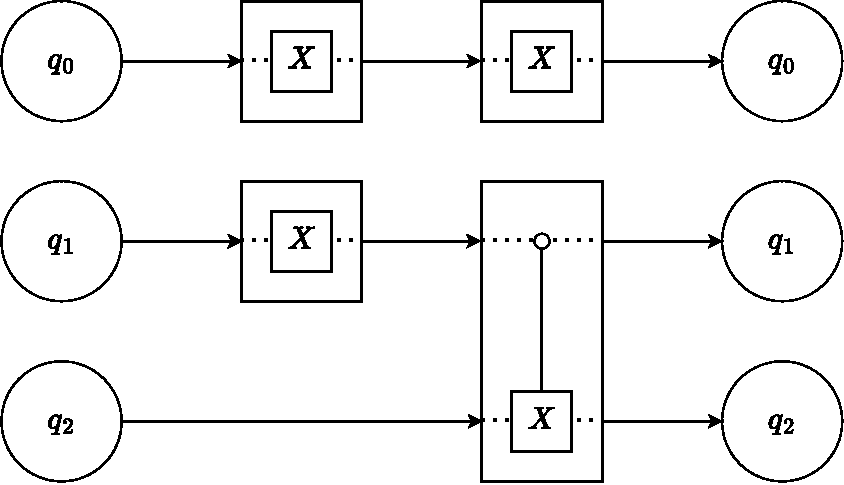
\includegraphics[width=\textwidth]{../figures/drawio/circuit_graph_optimized_firststep.pdf}
        \caption{Circuit graph after the first optimization.}
        \label{fig:circuit_graph_first_optimized}
    \end{minipage}
    \hfill
    \begin{minipage}{.35\textwidth}
        \centering     
        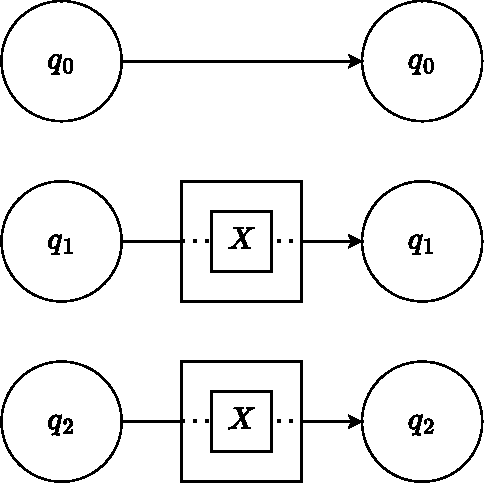
\includegraphics[width=\textwidth]{../figures/drawio/circuit_graph_optimized_complete.pdf}
        \caption{Completely optimized graph.}
        \label{fig:circuit_graph_optimized_complete}
    \end{minipage}
\end{figure}

In the next optimization round, the two $X$ gates on the first qubit wire are applied consecutively. Therefore, they can both be removed from the circuit. Finally, the combination of an $X$ gate child of an input node followed by a controlled-not gate can, again, be optimized such that the $CX$ gate is replaced with a simple $X$ gate on the third qubit wire. The result is a circuit where the first qubit remains unchanged and only an $X$ gate is applied to the second and third qubit. This result is also depicted in Fig~\ref{fig:circuit_graph_optimized_complete}. 

\subsubsection{Graph Translation}
After all possible optimizations rules were applied and no others were enabled in turn, the only remaining step is to translate the circuit graph back to a programmatic description. The qubits for the circuit are easily declared by iterating over all input or output nodes. Additionally, the qubit count can be reduced by leaving out all unused qubits, \ie no gates are applied to them. This is the case if the wire path only consists of the input and output nodes. In the case of the optimized circuit, depicted in Fig.~\ref{fig:circuit_graph_optimized_complete}, the first qubit $q_0$ can be skipped when adding the declarations to the translated program. 

For the gate applications, the only requirement is that, if a gate node is a descendent of another, its translated gate application statement must come after the statement of the ancestor node. Therefore, for most circuit graphs there are multiple possible programs describing the circuit correctly. For example, when translating the optimized graph described above, the order of the $X$ gate applications to both the second and third qubit is irrelevant such that both possibilities, \ie either applying the gate to $q_1$ or $q_2$ first, are valid translations of the program. Furthermore, while iterating over all input or output nodes and adding the corresponding qubit and register declarations to the beginning of the program is the easiest approach, the order and placement of the declarations is also arbitrary as long as they are declared before their first use. 

